%\documentclass[lang=cn,newtx,10pt,scheme=chinese]{elegantbook}
\documentclass[lang=cn,newtx,10pt,scheme=chinese,result=noanswer]{elegantbook}

\title{396数学基础讲义}
%\subtitle{Elegant\LaTeX\ 经典之作}

\author{Gaw}
\institute{HUAYAN}
\date{2026/9/1}
\version{0.1}
%\bioinfo{自定义}{信息}


\setcounter{tocdepth}{3}

\logo{logo-blue.png}
\cover{cover.jpg}

% 本文档命令
\usepackage{array}
\newcommand{\ccr}[1]{\makecell{{\color{#1}\rule{1cm}{1cm}}}}


% 修改标题页的橙色带
\definecolor{customcolor}{RGB}{32,178,170}
\colorlet{coverlinecolor}{customcolor}
\usepackage{cprotect}
\usepackage{exam-zh-choices}
\ExplSyntaxOn
\NewDocumentCommand{\fillparen}{o}
{
	\unskip \nobreak \hfill \penalty50 \hspace{1.5em} \hbox{} \nobreak \hfill
	\IfNoValueTF{#1}
	{（\hspace{0.9em} \hspace{0.9em}）} % 空括号内部左右各加 0.3em 空白
	{（\hspace{0.9em} \tl_trim_spaces:n {#1} \hspace{0.9em}）}
}
\ExplSyntaxOff

\usepackage{pifont}

\DeclareMathOperator{\arccot}{arccot}

\begin{document}

\maketitle
\frontmatter

\tableofcontents

\mainmatter

%% ------------高数部分-------------%%
%第1章 函数极限连续
\chapter{函数、极限与连续}

\begin{introduction}
	\item 函数
	\item 数列极限
	\item 函数极限
	\item 连续与间断
\end{introduction}

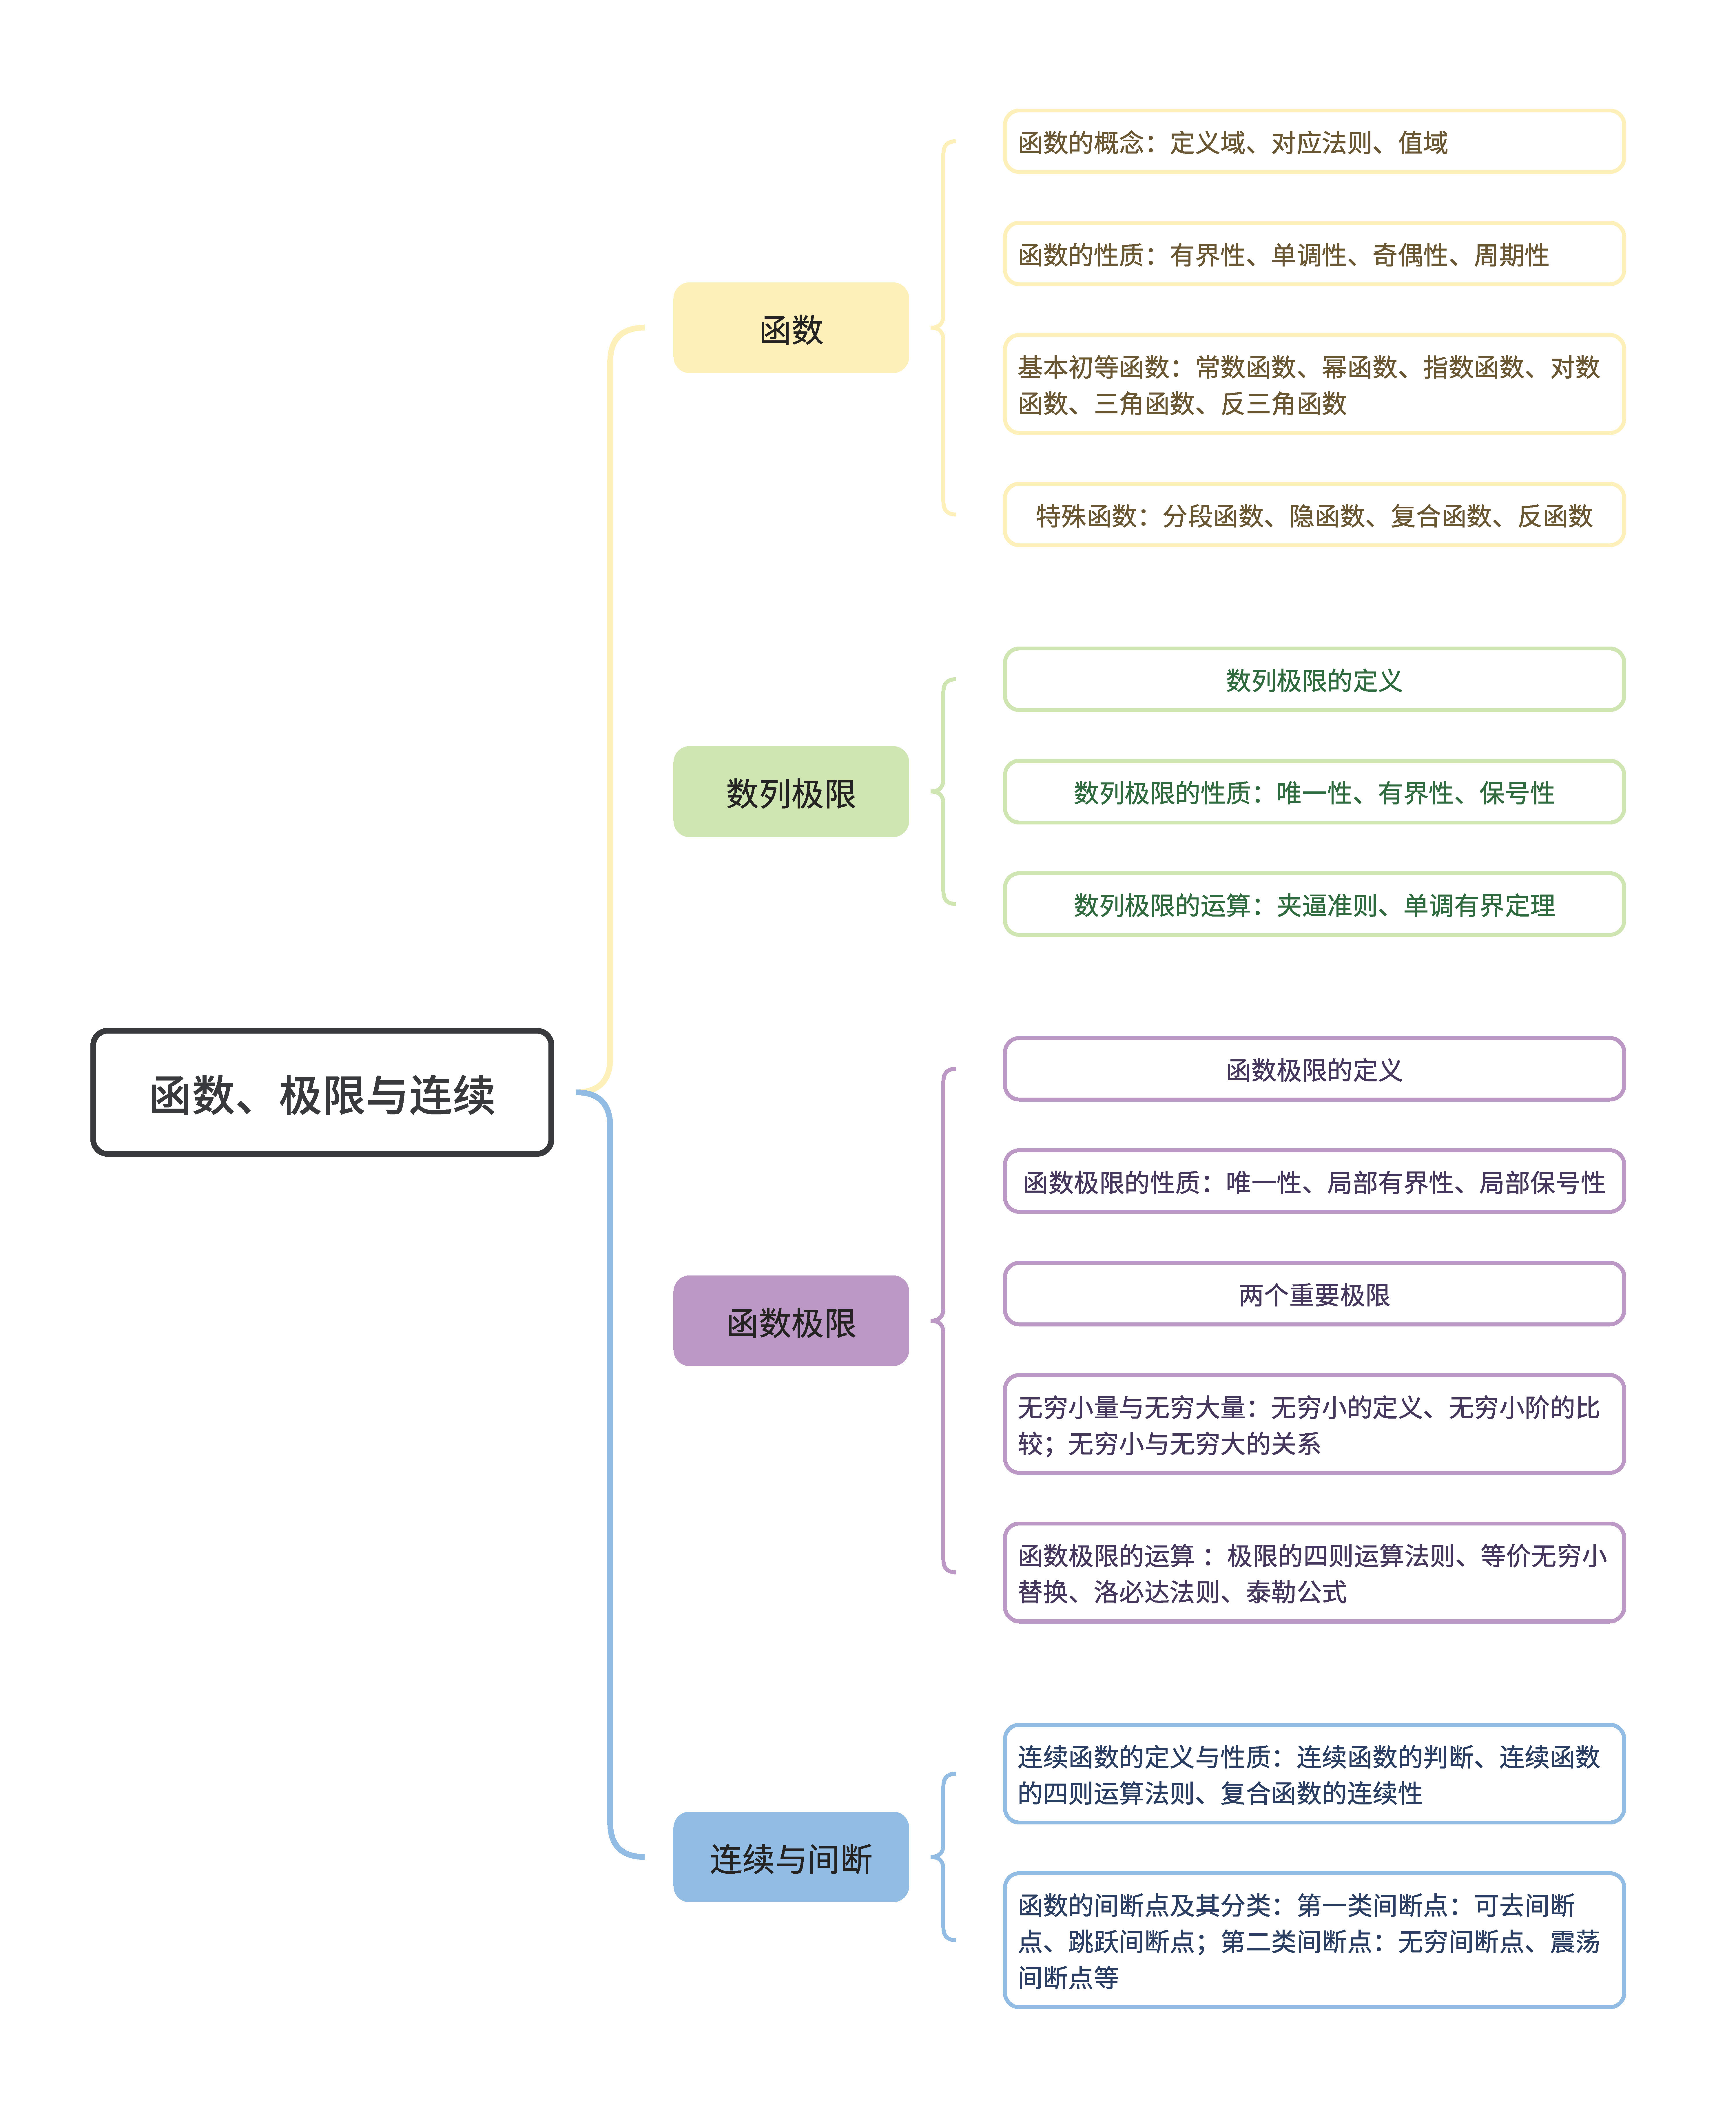
\includegraphics[width=16cm]{figure/chapter/chapter1.jpg}

\section{函数}
\subsection{函数的概念}
\begin{definition*}[函数]
    若 $D$ 为一个非空实数集合，设有一个对应法则 $f$ ，使得对每一个 $x \in D$ 都有唯一确定的实数 $y$ 与之对应，则称这个对应法则 $f$ 为定义在 $D$ 上的一个函数，或称变量 $y$ 是变量 $x$ 的函数，记作
$$
y=f(x), x \in D
$$
其中 $x$ 称为自变量，$y$ 称为因变量，集合 $D$ 称为函数的定义域，也可以记作 $D(f)$ ．对于 $x_0 \in D$ 所对应的 $y$ 的值，记作 $y_0$ 或 $f\left(x_0\right)$ ，称为当 $x=x_0$ 时函数 $y=f(x)$ 的函数值．全体函数值组成的集合 $\{y \mid y=f(x), x \in D\}$ 称为函数 $y=f(x)$ 的值域，记作 $f(D)$ ．	
\end{definition*}

\begin{remark}
	\begin{enumerate}
		\item 函数的三要素：定义域、对应法则、值域
		\item 两个函数相同：当且仅当两函数的定义域与对应法则完全相同．
		\item 函数定义域是指函数自变量的取值范围，例如函数 $f\left(x^2+5\right)$ 与 $f(x)$ 的自变量均为 $x$ .
		\item 在同一对应法则下，$f(\square)$ 括号内整体的取值范围是一样的．\\
	\end{enumerate}	
	
\end{remark}

% 1.1
\begin{example}
		
函数 $y=\sqrt{9-x^2}+\frac{1}{x}$ 的定义域为\fillparen[]
	\begin{choices}[columns=5]
		\item $[-3,0)$
		\item $(0,3]$
		\item $[-3,3]$
		\item $[-3,0) \cup(0,3]$
		\item $(0,9)$
	\end{choices}
	\vspace{3cm} 
\end{example}

\begin{solution}
 函数 $y=\sqrt{9-x^2}$ 的定义域为 $[-3,3]$ ，函数 $y=\frac{1}{x}$ 的定义域为 $(-\infty, 0) \cup(0, \infty)$ ，所以函数 $y=\sqrt{9-x^2}+\frac{1}{x}$ 的定义域为 $[-3,0) \cup(0,3]$ ,故应选D	
\end{solution}

%1.2
\begin{example}

设 $f(x)$ 的定义域为 $[5,10]$ ，则 $f\left(x^2+1\right)$ 的定义域为 
  \fillparen[ ]
	\begin{choices}[columns=5]
		\item $[-3,-2]$
		\item $［2，3］$
		\item $［－2，2］$
		\item $［－3，3 ］$
		\item $[-3,-2] \cup[2,3]$	
	\end{choices}
	\vspace{3cm} 
\end{example}
\begin{solution}
显然函数 $f(x)$ 中 $x$ 的取值范围为 $5 \leqslant x \leqslant 10$ ，又 $f\left(x^2+1\right)$ 中 $x^2+1$ 与 $f(x)$ 中 $x$ 的取值范围相同，所以 $5 \leqslant x^2+1 \leqslant 10$ ，解得 $-3 \leqslant x \leqslant-2$ 或 $2 \leqslant x \leqslant 3$ ，即 $f\left(x^2+1\right)$ 的定义域为$[-3,-2] \cup[2,3]$ ，故应选 E．
\end{solution}


%1.3
\begin{example}
	
若函数 $y=f(x+1)$ 的定义域是 $[-2,3]$ ，则函数 $y=f(2 x-1)$ 的定义域为
	\fillparen[ ]
	\begin{choices}[columns=5]
		\item $[0,3]$
		\item $[-2,4]$
		\item $\left[-5, \frac{5}{2}\right]$
		\item $\left[-1, \frac{4}{5}\right]$
		\item $\left[0, \frac{5}{2}\right]$
	\end{choices}
	%\vspace{3cm} 
\end{example}
\begin{solution}
因为函数 $y=f(x+1)$ 的定义域是 $[-2,3]$ ，即 $-2 \leqslant x \leqslant 3,-1 \leqslant x+1 \leqslant 4$ ，所以函数 $y=f(x)$ 的定义域为 $[-1,4]$。

	
对于函数 $y=f(2 x-1),-1 \leqslant 2 x-1 \leqslant 4,0 \leqslant x \leqslant \frac{5}{2}$ ，所以函数 $y=f(2 x-1)$ 的定义域为 $\left[0, \frac{5}{2}\right]$ ，故应选E
\end{solution}

\newpage


\subsection{函数的性质}
\noindent \textbf{一、有界性}
\begin{definition*}[有界性]
设 $f$ 为定义在 $D$ 上的函数．若存在正数 $M$ ，使得对每一个 $x \in D$ ，有
$$
	|f(x)| \leqslant M
$$
则称 $f$ 为 $D$ 上的有界函数．	
\end{definition*}


\begin{remark}
	\begin{enumerate}
		\item 函数 $f(x)$ 有界或无界是相对于某个区间而言的
		\item 函数有界的充要条件是函数既有上界又有下界\\
	\end{enumerate}
\end{remark}

\noindent \textbf{二、单调性}
\begin{definition*}[单调性]
设 $f$ 为定义在 $D$ 上的函数．若对任何 $x_1, x_2 \in D$ ，当 $x_1<x_2$ 时，总有
\begin{itemize}
	\item[（i）] $f\left(x_1\right) \leqslant f\left(x_2\right)$ ，则称 $f$ 为 $D$ 上的（递）增函数，特别当成立严格不等式 $f\left(x_1\right)< f\left(x_2\right)$ 时，称 $f$ 为 $D$ 上的严格（递）增函数；
	\item[（ii）] $f\left(x_1\right) \geqslant f\left(x_2\right)$ ，则称 $f$ 为 $D$ 上的（递）减函数，特别当成立严格不等式 $f\left(x_1\right)> f\left(x_2\right)$ 时，称 $f$ 为 $D$ 上的严格（递）减函数；
\end{itemize}

增函数和减函数统称为单调函数，严格增函数和严格减函数统称为严格单调函数．	\\
\end{definition*}


\noindent \textbf{三、奇偶性}
\begin{definition*}[奇偶性]
设 $D$ 为对称于原点的数集，$f$ 为定义在 $D$ 上的函数．若对每一个 $x \in D$ ，有
$$
f(-x)=-f(x)(\quad f(-x)=f(x)\quad )
$$
则称 $f$ 为 $D$ 上的奇（偶）函数。

从函数图形上看，奇函数的图像关于原点对称，偶函数的图像则关于 $y$ 轴对称．	
\end{definition*}


\begin{remark}
	\begin{enumerate}
		\item 若奇函数 $f(x)$ 在 $x=0$ 处有定义，则 $f(0)=0$ 
		\item 奇 $\pm$ 奇 = 奇，偶 $\pm$ 偶 = 偶,奇 $\times$ 奇 = 偶，偶 $\times$ 偶 = 偶,奇 $\times$ 偶 = 奇．\\
	\end{enumerate}
\end{remark}

\begin{example}
		
函数 $f(x)=\ln \left(\sqrt{x^2+a^2}+x\right)(a$ 为常数，且 $a \neq 0)$ \fillparen[ ]
	\begin{choices}[columns=3]
		\item 为奇函数
		\item 为偶函数
		\item 当 $a= \pm 1$ 时为奇函数
		\item 当 $a= \pm 1$ 时为偶函数
		\item 为非奇非偶函数	
	\end{choices}
	\vspace{3cm} 
\end{example}
\begin{solution}
由 $f(x)=\ln \left(\sqrt{x^2+a^2}+x\right)$ ，得

$$
\begin{aligned}
	f(-x) & =\ln \left[\sqrt{(-x)^2+a^2}-x\right]=\ln \left(\sqrt{x^2+a^2}-x\right) \\
	& =\ln \frac{\left(\sqrt{x^2+a^2}-x\right)\left(\sqrt{x^2+a^2}+x\right)}{\sqrt{x^2+a^2}+x}=\ln \frac{a^2}{\sqrt{x^2+a^2}+x} \\
	& =\ln a^2-\ln \left(\sqrt{x^2+a^2}+x\right)
\end{aligned}
$$

可知当 $a^2=1$ ，即 $a= \pm 1$ 时， $\ln a^2=0$ ，从而

$$
f(-x)=-\ln \left(\sqrt{x^2+a^2}+x\right)=-f(x),
$$

此时 $f(x)$ 为奇函数．当 $a^2 \neq 1$ ，即 $a \neq \pm 1$ 时，$f(x)$ 为非奇非偶函数．故选（C）．	
\end{solution}
\newpage


\begin{example}
	
以下四个函数	
	\begin{equation*}  
		f_1(x)=\frac{\mathrm{e}^x+\mathrm{e}^{-x}}{2} ,f_2(x)=\frac{\mathrm{e}^x-\mathrm{e}^{-x}}{2} , f_3(x)=\ln \frac{1-x}{1+x} ,f_4(x)=\ln \left(x+\sqrt{x^2+1}\right)   
	\end{equation*} 
其中是奇函数的个数是	\fillparen[ ]
	\begin{choices}[columns=5]
		\item 0
		\item 1
		\item 2
		\item 3
		\item 4	
	\end{choices}
	\vspace{3cm} 
\end{example}
\begin{solution}
显然题设中四个函数的定义域均关于原点对称，因为
$$
\begin{aligned}
	f_1(-x) & =\frac{\mathrm{e}^{-x}+\mathrm{e}^x}{2}=f_1(x), \text { 即 } f_1(x) \text { 为偶函数; } \\
	f_2(-x) & =\frac{\mathrm{e}^{-x}-\mathrm{e}^x}{2}=-f_2(x), \text { 即 } f_2(x) \text { 为奇函数; } \\
	f_3(-x) & =\ln \frac{1+x}{1-x}=-\ln \frac{1-x}{1+x}=-f_3(x), \text { 即 } f_3(x) \text { 为奇函数; } \\
	f_4(-x) & =\ln \left(-x+\sqrt{x^2+1}\right)=\ln \frac{1}{\sqrt{x^2+1}+x} \\
	& =-\ln \left(x+\sqrt{x^2+1}\right)=-f_4(x), \text { 即 } f_4(x) \text { 为奇函数, }
\end{aligned}
$$
所以奇函数的个数为 3，故应选 D．	
\end{solution}


\noindent \textbf{四、周期性}
\begin{definition*}[周期性]
设函数 $f(x)$ 的定义域为 $D$ ，若存在一个正数 $T$ ，使得对于任意 $x \in D$ ，有 $x+T \in D$ ，且 $$f(x+ T)=f(x)$$则称 $f(x)$ 为周期函数，且正数 $T$ 为 $f(x)$ 的周期．	
\end{definition*}
易知，若 $T$为 $f(x)$ 的一个周期，则对任意的整数 $n, n T$ 亦为 $f(x)$ 的周期．在 $f(x)$ 的所有周期中，我们把其中最小的正数称为最小正周期．通常我们所说周期函数的周期是指最小正周期．

并不是所有的周期函数都有周期．例如：狄利克雷函数
$$
D(x)= \begin{cases}1, & x \text { 为有理数 } \\ 0, & x \text { 为无理数 }\end{cases}
$$
任意正实数都是周期，但不存在最小正实数，所以这个函数没有周期．


常见的周期函数： $\sin x, \cos x$ 均为周期为 $2 \pi$ 的周期函数； $\tan x, \cot x$ 均为周期为 $\pi$ 的周期函数．


\begin{remark}
	\begin{enumerate}
		\item 如果函数 $f_1(x), f_2(x)$ 都以 $T$ 为周期，则 $k_1 f_1(x)+k_2 f_2(x)$ 仍然以 $T$ 为周期
		\item 如果函数 $f_1(x), f_2(x)$ 分别以 $T_1, T_2$ 为周期，则 $f_1(x) \pm f_2(x)$ 也是周期函数，其周期为 $T_1$ 和 $T_2$ 的最小公倍数\\
	\end{enumerate}
\end{remark}


\begin{example}
		
若 $f(x)$ 既关于直线 $x=a$ 对称，又关于直线 $x=b$ 对称，且 $b>a$ ，则 $f(x)$ 的周期为	\fillparen[ ]
	\begin{choices}[columns=5]
		\item $a$
		\item $a+b$
		\item $b-a$
		\item $b$
		\item $2 b-2 a$	
	\end{choices}
	\vspace{3cm} 
\end{example}
\begin{solution}
$f(x)$ 关于直线 $x=a$ 对称得到 $f(a-x)=f(a+x)$ ，可以化为 $f(t)=f(2 a-t)$ ；$f(x)$ 关于直线 $x=b$ 对称得到 $f(b-x)=f(b+x)$ ，可以化为 $f(t)=f(2 b-t)$ ．综合以上两式得到 $f(2 a-t)=f(2 b-t) \Rightarrow f(u)=f(u+2(b-a))$ ，故周期为 $2 b-2 a$ ，故选 E．	
\end{solution}

\newpage

\subsection{基础初等函数}
常数函数、幂函数、指数函数、对数函数、三角函数、反三角函数统称为基本初等函数


\textbf{一、常值函数}


$y=C$ ，定义域为 $(-\infty,+\infty)$ ，图形为平行于 $x$ 轴的直线．在 $y$ 轴上的截距为 $C$ ．


\begin{center}
	\begin{tikzpicture}[scale=0.6]
		% 对称的坐标轴
		\draw[->] (-5,0) -- (5,0) node[below] {\(x\)};
		\draw[->] (0,-3) -- (0,3) node[left] {\(y\)};
		\node at (0,0) [below left] {\(O\)};
		
		% 绘制两条粗细一样的天蓝色水平线，标签统一放在右侧
		\draw[cyan, thick] (-4, 2) -- (4, 2) node[right] {\(y=C \ (C>0)\)};
		\draw[cyan, thick] (-4, -2) -- (4, -2) node[right] {\(y=C \ (C<0)\)};
		
		% 在 x 轴右侧标注 C=0
		\node at (6, 0) {\(C=0\)};
	\end{tikzpicture}
\end{center}

\textbf{二、幂函数}


$y=x^a$ ，其定义域随着 $\alpha$ 的不同而变化．但不论 $\alpha$ 取何值，总在 $(0,+\infty)$ 内有定义，且
图形过点 $(1,1)$ ．当 $\alpha>0$ 时，函数图形过原点．

\begin{center}
	\begin{tikzpicture}[scale=0.8]
		% 坐标轴 (为了容纳 y=x^3，将Y轴范围拉大)
		\draw[->] (-5,0) -- (5,0) node[below] {\(x\)};
		\draw[->] (0,-3.5) -- (0,3.5) node[left] {\(y\)};
		\node at (0,0) [below left] {\(O\)};
		
		
		% y = x^2 (蓝色粗线)
		\draw[cyan, thick, domain=-1.5:1.5, samples=100] plot (\x, {\x*\x});
		\node at (-1.8, 2.5) {\(y=x^2\)}; % 标签放在曲线的左上侧
		
		% y = x (黑色粗线)
		\draw[black, thick, domain=-2.5:2.5, samples=100] plot (\x, {\x});
		\node at (3.5, 3) {\(y=x\)}; % 标签放在直线的右上侧
		
		% y = x^(1/2) (黑色粗线) 注意定义域 x >= 0
		\draw[orange, thick, domain=0:3.5, samples=100] plot (\x, {sqrt(\x)});
		\node at (5.0, 2) {\(y=x^{1/2}\)}; % 标签放在曲线的右上方
		
		% y = 1/x (黑色粗线) 注意分段绘制，避免 x=0 处连线
		\draw[green!50, thick, domain=0.3:3.5, samples=100] plot (\x, {1/\x});
		\node at (5.0, 0.4) {\(y=1/x\)};
		\draw[green!50, thick, domain=-3.5:-0.3, samples=100] plot (\x, {1/\x});
		\node at (-5.0, -0.4) {\(y=1/x\)};
	
	\end{tikzpicture}
\end{center}



\textbf{三、指数函数}


$y=a^x(a>0, a \neq 1)$ ，其定义域为 $(-\infty,+\infty)$ 。当 $0<a<1$ 时，函数严格单调递减;当 $a>1$ 时，函数严格单调递增．指数函数的图形恒过点$(0,1)$。微积分中经常用到以 $e$为底的指数函数，即 $y=\mathrm{e}^x$.指数函数 $y=a^x$ 的性质归纳见下表。



\begin{tabular}[t]{|c|c|c|}
	\hline & \(a>1\) & \(0<a<1\) \\
	\cline{2-3} % 关键修改：只画2、3列的横线
	\multirow{6}{*}{\shortstack{图像 \\[15ex] 性质}} &  \centering \resizebox{4cm}{!}{
		\begin{tikzpicture}[>=stealth, font=\large]
			\definecolor{skyblue}{RGB}{0, 158, 224}
			\draw[->, thick, gray!80!black] (-2.5,0) -- (2.5,0) node[below=1pt, xshift=-2pt] {\(x\)};
			\draw[->, thick, gray!80!black] (0,-0.5) -- (0,3.5) node[left=1pt] {\(y\)};
			\node[below left=1pt, inner sep=1pt] at (0,0) {\(O\)};
			\draw[skyblue, very thick, domain=-1.8:1.5, samples=100] plot (\x, {2^\x});
		\end{tikzpicture}
	}  &  \resizebox{4cm}{!}{
		\begin{tikzpicture}[>=stealth, font=\large]
			\definecolor{skyblue}{RGB}{0, 158, 224}
			\draw[->, thick, gray!80!black] (-2.5,0) -- (2.5,0) node[below=1pt, xshift=-2pt] {\(x\)};
			\draw[->, thick, gray!80!black] (0,-0.5) -- (0,3.5) node[left=1pt] {\(y\)};
			\node[below left=1pt, inner sep=1pt] at (0,0) {\(O\)};
			\draw[skyblue, very thick, domain=-1.5:1.5, samples=100] plot (\x, {0.5^\x});
		\end{tikzpicture}
	} 	
	\\
	\cline{2-3} % 关键修改：只画2、3列的横线
	& \multicolumn{2}{|l|}{（1）定义域： $\mathbf{R}$} \\
	\cline{2-3}
	& \multicolumn{2}{|l|}{（2）值域：$(0,+\infty)$ ，图像在 $x$ 轴上方} \\
	\cline{2-3}
	&  \multicolumn{2}{|l|}{ （3）过点（0，1），即 $x=0$ 时，$y=1$ } \\   
	\cline{2-3}
	& （4）当 $a>1$ 时，$\left\{\begin{array}{l}\text { 若 } x>0, \text { 则 } a^x>1 \\ \text { 若 } x<0, \text { 则 } 0<a^x<1\end{array}\right.$ & 当 $0<a<1$ 时，$\left\{\begin{array}{l}\text { 若 } x<0, \text { 则 } a^x>1 \\ \text { 若 } x>0, \text { 则 } 0<a^x<1\end{array}\right.$ \\
	\cline{2-3}
	& （5）在 $\mathbf{R}$ 上是增函数 & 在 $\mathbf{R}$ 上是减函数 \\
	\hline
\end{tabular}
\\

\textbf{四、对数函数}


$y=\log _a x(a>0, a \neq 1)$ ，其定义域为 $(0,+\infty)$ ，它与 $y=a^x$ 互为反函数．微积分中常用到以 e 为底的对数，记作 $y=\ln x$ ，称为自然对数．对数函数的图形恒过点 $(1,0)$ ．对数函数$y=\log _a x$ 的性质归纳见下表．


\begin{tabular}[t]{|c|p{6.8cm}|p{6.8cm}|}
	\hline & \centering \(a>1\) & \(0<a<1\) \\
	\cline{2-3} % 关键修改：只画2、3列的横线
	\multirow{5}{*}{\shortstack{图像 \\[10ex] 性质}} &  \centering \resizebox{4cm}{!}{
		\begin{tikzpicture}[>=stealth, font=\large]
			\definecolor{skyblue}{RGB}{0, 158, 224}
			\draw[->, thick, gray!80!black] (-1.5,0) -- (4.5,0) node[below=1pt, xshift=-2pt] {\(x\)};
			\draw[->, thick, gray!80!black] (0,-2.5) -- (0,2.5) node[left=1pt] {\(y\)};
			\node[below left=1pt, inner sep=1pt] at (0,0) {\(O\)};
			\node[below right] at (1,0) {\(1\)};
			\draw[skyblue, very thick, domain=0.2:4.5, samples=100] plot (\x, {ln(\x)});
			\draw[dashed] (1,-2.5) -- (1,2.5);
		\end{tikzpicture}
	}  &  \resizebox{4cm}{!}{
		\begin{tikzpicture}[>=stealth, font=\large]
			\definecolor{skyblue}{RGB}{0, 158, 224}
			\draw[->, thick, gray!80!black] (-1.5,0) -- (4.5,0) node[below=1pt, xshift=-2pt] {\(x\)};
			\draw[->, thick, gray!80!black] (0,-2.5) -- (0,2.5) node[left=1pt] {\(y\)};
			\node[below left=1pt, inner sep=1pt] at (0,0) {\(O\)};
			\node[below right] at (1,0) {\(1\)};
			\draw[skyblue, very thick, domain=0.2:4.5, samples=100] plot (\x, {ln(\x)/ln(0.5)});  % log_{0.5} x
			\draw[dashed] (1,-2.5) -- (1,2.5);
		\end{tikzpicture}	
	} 	
	\\
	\cline{2-3} % 关键修改：只画2、3列的横线
	& \multicolumn{2}{|l|}{（1）定义域：$(0,+\infty)$，图像在 $y$ 轴右侧}\\
	\cline{2-3}
	& \multicolumn{2}{|l|}{（2）值域： $\mathbf{R}$ } \\
	\cline{2-3}
	& \multicolumn{2}{|l|}{ （3）过点（1，0），即 $x=1$ 时，$y=0$} \\  
	\cline{2-3}
	& （4）在 $(0,+\infty)$上是增函数 & 在 $(0,+\infty)$上是减函数 \\
	\hline
\end{tabular}
\vspace{0.8cm}

\textbf{五、三角函数}


常用的三角函数见下表.


\begin{tabular}[t]{|>{\centering\arraybackslash}m{1.2cm}|>{\centering\arraybackslash}m{3.5cm}|>{\centering\arraybackslash}m{3.5cm}|>{\centering\arraybackslash}m{3.5cm}|>{\centering\arraybackslash}m{3.5cm}|}
	\hline & \centering $y=\sin x$ & $y=\cos x$ & $y=\tan x$ & $y=\cot x$ \\
	\hline 定义域 & R & R & $x \neq k \pi+\frac{\pi}{2}(k \in \mathbf{Z})$ & $x \neq k \pi(k \in \mathbf{Z})$ \\
	\hline 值域 & $[-1,1]$ & $[-1,1]$ & R & R \\
	\hline  \makecell[c]{图像}
	& \resizebox{3.5cm}{!}{
		\begin{tikzpicture}[>=stealth, font=\large]
		\definecolor{skyblue}{RGB}{0, 158, 224}
		
		% 坐标轴
		\draw[->, thick, gray!80!black] (-3.5,0) -- (3.5,0) node[below right] {\(x\)};
		\draw[->, thick, gray!80!black] (0,-3.5) -- (0,3.5) node[left] {\(y\)};
		
		% 正弦曲线：domain 直接使用 -pi 到 pi，sin(\x r) 将弧度转为度数
		\draw[skyblue, very thick, domain=-pi:pi, samples=100] plot (\x, {sin(\x r)});
		\end{tikzpicture}
	}	
	& 
	\resizebox{3.5cm}{!}{
		\begin{tikzpicture}[>=stealth, font=\large]
			\definecolor{skyblue}{RGB}{0, 158, 224}
			
			% 坐标轴
			\draw[->, thick, gray!80!black] (-3.5,0) -- (3.5,0) node[below right] {\(x\)};
			\draw[->, thick, gray!80!black] (0,-3.5) -- (0,3.5) node[left] {\(y\)};

			
			% 正弦曲线：domain 直接使用 -pi 到 pi，sin(\x r) 将弧度转为度数
			\draw[skyblue, very thick, domain=-pi:pi, samples=100] plot (\x, {cos(\x r)});
		\end{tikzpicture}
	}

	& 
	\resizebox{3.5cm}{!}{
		\begin{tikzpicture}[>=stealth, font=\large]
			\definecolor{skyblue}{RGB}{0, 158, 224}
			
			% 坐标轴
			\draw[->, thick, gray!80!black] (-3.5,0) -- (3.5,0) node[below right] {\(x\)};
			\draw[->, thick, gray!80!black] (0,-3.5) -- (0,3.5) node[left] {\(y\)};

			
			% 渐近线（虚线）
			\draw[dashed, gray!60] (-1.5708,-3.5) -- (-1.5708,3.5);
			\draw[dashed, gray!60] (1.5708,-3.5) -- (1.5708,3.5);
			
			% 绘制正切曲线，裁剪 y 轴范围以显示有限区域
			\begin{scope}
				\clip (-2.8,-3.5) rectangle (2.8,3.5);
				\draw[skyblue, very thick, domain=-pi/2+0.03:pi/2-0.03, samples=200] plot (\x, {tan(\x r)});
			\end{scope}
		\end{tikzpicture}
	}
	& 
	\resizebox{3.5cm}{!}{
		\begin{tikzpicture}[>=stealth, font=\large]
			\definecolor{skyblue}{RGB}{0, 158, 224}
			
			% 坐标轴（适当扩大范围）
			\draw[->, thick, gray!80!black] (-3.5,0) -- (3.5,0) node[below right] {\(x\)};
			\draw[->, thick, gray!80!black] (0,-3.5) -- (0,3.5) node[left] {\(y\)};
			\node[below left=1pt, inner sep=1pt] at (0,0) {\(O\)};
			
			
			% 渐近线（虚线）
			\draw[dashed, gray!60] (-3.1416,-3.5) -- (-3.1416,3.5);
			\draw[dashed, gray!60] (0,-3.5) -- (0,3.5);
			\draw[dashed, gray!60] (3.1416,-3.5) -- (3.1416,3.5);
			
			% 绘制 cotx 的两个分支，避开奇点
			\begin{scope}
				\clip (-3.5,-3.5) rectangle (3.5,3.5);  % 裁剪超出部分
				\draw[skyblue, very thick, domain=-pi+0.03:-0.03, samples=200] 
				plot (\x, {cos(\x r)/sin(\x r)});
				\draw[skyblue, very thick, domain=0.03:pi-0.03, samples=200] 
				plot (\x, {cos(\x r)/sin(\x r)});
			\end{scope}
		\end{tikzpicture}
	}
	\\
	\hline 周期性 & $2 \pi$ & $2 \pi$ & $\boldsymbol{\pi}$ & $\pi$ \\
	\hline 奇偶性 & 奇函数 & 偶函数 & 奇函数 & 奇函数 \\
	\hline \makecell{单调性} & \begin{tabular}[t]{c}
		$\left[2 k \pi-\frac{\pi}{2}, 2 k \pi+\frac{\pi}{2}\right]$  $\uparrow$
		\\
		$[2 k \pi+\frac{\pi}{2}, 2 k \pi+\frac{3 \pi}{2}]$  $\downarrow$
	\end{tabular} & \begin{tabular}[t]{c}
		$[(2 k-1) \pi, 2 k \pi]$ \quad $\uparrow$
		\\
		$[2 k \pi,(2 k+1) \pi]$ \quad $\downarrow$
		
	\end{tabular} & \begin{tabular}[t]{c}
		$\left(k \pi-\frac{\pi}{2}, k \pi+\frac{\pi}{2}\right)$
		\quad $\uparrow$
	\end{tabular} & \begin{tabular}[t]{c}
		$(k \pi,(k+1) \pi)$
		\quad $\downarrow$
	\end{tabular} \\
	\hline
\end{tabular}

\vspace{0.5cm}
特殊角的三角函数值见下表．

\begingroup
\renewcommand{\arraystretch}{1.8}
\setlength{\extrarowheight}{0pt} 
\begin{tabular}[t]{|>{\centering\arraybackslash}m{2cm}|>{\centering\arraybackslash}m{2cm}|>{\centering\arraybackslash}m{2cm}|>{\centering\arraybackslash}m{2cm}|>{\centering\arraybackslash}m{2cm}|>{\centering\arraybackslash}m{2cm}|}
	\hline $\alpha$ & \color{red}{0} & \color{red}{ $\frac{\pi}{6}$ }  & \color{red}{ $\frac{\pi}{4}$ }  & \color{red}{ $\frac{\pi}{3}$ }  & \color{red}{ $\frac{\pi}{2}$ }  \\
	\hline $\sin \alpha$ & 0 & $\frac{1}{2}$ & $\frac{\sqrt{2}}{2}$ & $\frac{\sqrt{3}}{2}$ & 1 \\
	\hline $\cos \alpha$ & 1 & $\frac{\sqrt{3}}{2}$ & $\frac{\sqrt{2}}{2}$ & $\frac{1}{2}$ & 0 \\
	\hline $\tan \alpha$ & 0 & $\frac{\sqrt{3}}{3}$ & 1 & $\sqrt{3}$ & 不存在 \\
	\hline $\cot \alpha$ & 不存在 & $\sqrt{3}$ & 1 & $\frac{\sqrt{3}}{3}$ & 0 \\
	\hline
\end{tabular}

\endgroup

\newpage

\textbf{六、反三角函数函数}


常用的反三角函数：


\begin{tabular}[t]{|>{\centering\arraybackslash}m{1.2cm}|>{\centering\arraybackslash}m{3.5cm}|>{\centering\arraybackslash}m{3.5cm}|>{\centering\arraybackslash}m{3.5cm}|>{\centering\arraybackslash}m{3.5cm}|}
	\hline & \centering $y=\arcsin x$ & $y=\arccos x$ & $y=\arctan x$ & $y=\arccot x$ \\
	\hline 定义域 & $[-1,1]$ & $[-1,1]$ & R &  R\\
	\hline 值域 & $[-\frac{\pi}{2},\frac{\pi}{2}]$ & $
	[0,\pi]$ & $(-\frac{\pi}{2},\frac{\pi}{2})$ & $(0,\pi)$ \\
	\hline  \makecell[c]{图像}
	& \resizebox{3.5cm}{!}{
	\begin{tikzpicture}[>=stealth, font=\large]
		\definecolor{skyblue}{RGB}{0, 158, 224}
		
		% 坐标轴
		\draw[->, thick, black] (-1.5,0) -- (1.5,0) node[below right] {\(x\)};
		\draw[->, thick, black] (0,-2.2) -- (0,2.2) node[left] {\(y\)};
		
		% 绘制 arcsin x（参数方程）
		\draw[skyblue, very thick, domain=-pi/2:pi/2, samples=100] plot ({sin(\x r)}, \x);
		
		% 添加水平虚线 y = π/2 和 y = -π/2（仅画在定义域 x∈[-1,1] 内）
		\draw[dashed, skyblue, thick] (0, {pi/2}) -- (1, {pi/2});
		\draw[dashed, skyblue, thick] (-1, {-pi/2}) -- (0, {-pi/2});
		
		% 刻度标签（可选）
		\node[below] at (1,0) {1};
		\node[below] at (-1,0) {-1};
		\node[left] at (0,1.57) {\(\frac{\pi}{2}\)};
		\node[left] at (0.8,-1.57) {\(-\frac{\pi}{2}\)};
	\end{tikzpicture}
	}	
	& 
	\resizebox{3.5cm}{!}{
	\begin{tikzpicture}[>=stealth, font=\large]
		\definecolor{skyblue}{RGB}{0, 158, 224}
		
		% 坐标轴
		\draw[->, thick, black] (-1.5,0) -- (1.5,0) node[below right] {\(x\)};
		\draw[->, thick, black] (0,-0.5) -- (0,4.0) node[left] {\(y\)};
		
		\draw[dashed, skyblue, thick] (-1, {pi}) -- (0, {pi});
		
				
		% 刻度（可选）
		\draw (-1,0) -- (-1,-0.1) node[below] {\(-1\)};
		\draw (1,0) -- (1,-0.1) node[below] {\(1\)};
		\draw (0,{pi/2}) -- (-0.2,{pi/2}) node[left] {\(\frac{\pi}{2}\)};
		\draw (0,{pi}) -- (-0.1,{pi})
		node[right] at (0.15,3.14) {\(\pi\)};
		
		% 反余弦曲线：y = arccos(x)
		\draw[skyblue, very thick, domain=-1:1, samples=100] plot (\x, {rad(acos(\x))});
	\end{tikzpicture}
	}
	
	& 
	\resizebox{3.5cm}{!}{

	\begin{tikzpicture}[>=stealth, font=\large]
		\definecolor{skyblue}{RGB}{0, 158, 224}
		
		% 坐标轴
		\draw[->, thick, black] (-2,0) -- (2,0) node[below right] {\(x\)};
		\draw[->, thick, black] (0,-2.5) -- (0,2.5) node[left] {\(y\)};
		
		% 水平渐近线（虚线）
		\draw[dashed, black] (-2,{pi/2}) -- (2,{pi/2}) node[right] {\(\frac{\pi}{2}\)};
		\draw[dashed, black] (-2,{-pi/2}) -- (2,{-pi/2}) node[right] {\(-\frac{\pi}{2}\)};
		
		% 绘制反正切曲线（无需裁剪）
		\draw[skyblue, very thick, domain=-2:2, samples=200] plot (\x, {rad(atan(\x))});
	\end{tikzpicture}
	}
	& 
	\resizebox{3.5cm}{!}{

	\begin{tikzpicture}[>=stealth, font=\large]
		\definecolor{skyblue}{RGB}{0, 158, 224}
		
		% 坐标轴（x 轴加宽，y 轴上提以显示渐近线）
		\draw[->, thick, black] (-2,0) -- (2,0) node[below right] at (1.5,0) {\(x\)};
		\draw[->, thick, black] (0,-0.5) -- (0,3.5) node[left] {\(y\)};

		
		% 水平渐近线（虚线）
		\draw[dashed, black] (-2,0) -- (2,0) node[right] {\(0\)};
		\draw[dashed, black] (-2,{pi}) -- (2,{pi}) node[right] {\(\pi\)};
		
		% 绘制 arccot 曲线（单调递减，从 π 到 0）
		\draw[skyblue, very thick, domain=-2:2, samples=200] 
		plot (\x, {pi/2 - rad(atan(\x))});
	\end{tikzpicture}
	}
	\\
	\hline 奇偶性 & 奇函数 & 非奇非偶函数 & 奇函数 & 非奇非偶函数 \\
	\hline \makecell{单调性} & 在定义域内是增函数&在定义域内是减函数 & 在定义域内是增函数 & 在定义域内是减函数 \\
	\hline
\end{tabular}


\subsection{特殊函数}
\textbf{一、常值函数}


\begin{example}
	
	
	\fillparen[ ]
	\begin{choices}[columns=5]
		\item 
		\item 
		\item 
		\item 
		\item 	
	\end{choices}
	\vspace{3cm} 
\end{example}
\begin{solution}
	
\end{solution}

\section{数列极限}
\subsection{数列极限的定义}
\subsection{数列极限的性质}
\subsection{数列极限的运算}

\section{函数极限}
\subsection{函数极限的定义}
\subsection{函数极限的性质}
\subsection{两个重要极限}
\subsection{无穷小量与无穷大量}
\subsection{函数极限的运算}
\section{连续与间断}
\subsection{连续函数的定义与性质}
\subsection{函数的间断点及其分类}

\begin{example}
	
	
	\fillparen[ ]
	\begin{choices}[columns=5]
		\item 
		\item 
		\item 
		\item 
		\item 	
	\end{choices}
	\vspace{3cm} 
\end{example}
\begin{solution}
	
\end{solution}

%第2章 一元函数微分学
\chapter{一元函数微分学}

\begin{introduction}
	\item 导数
	\item 微分
	\item 导数应用
	\item 微分中值定理
\end{introduction}

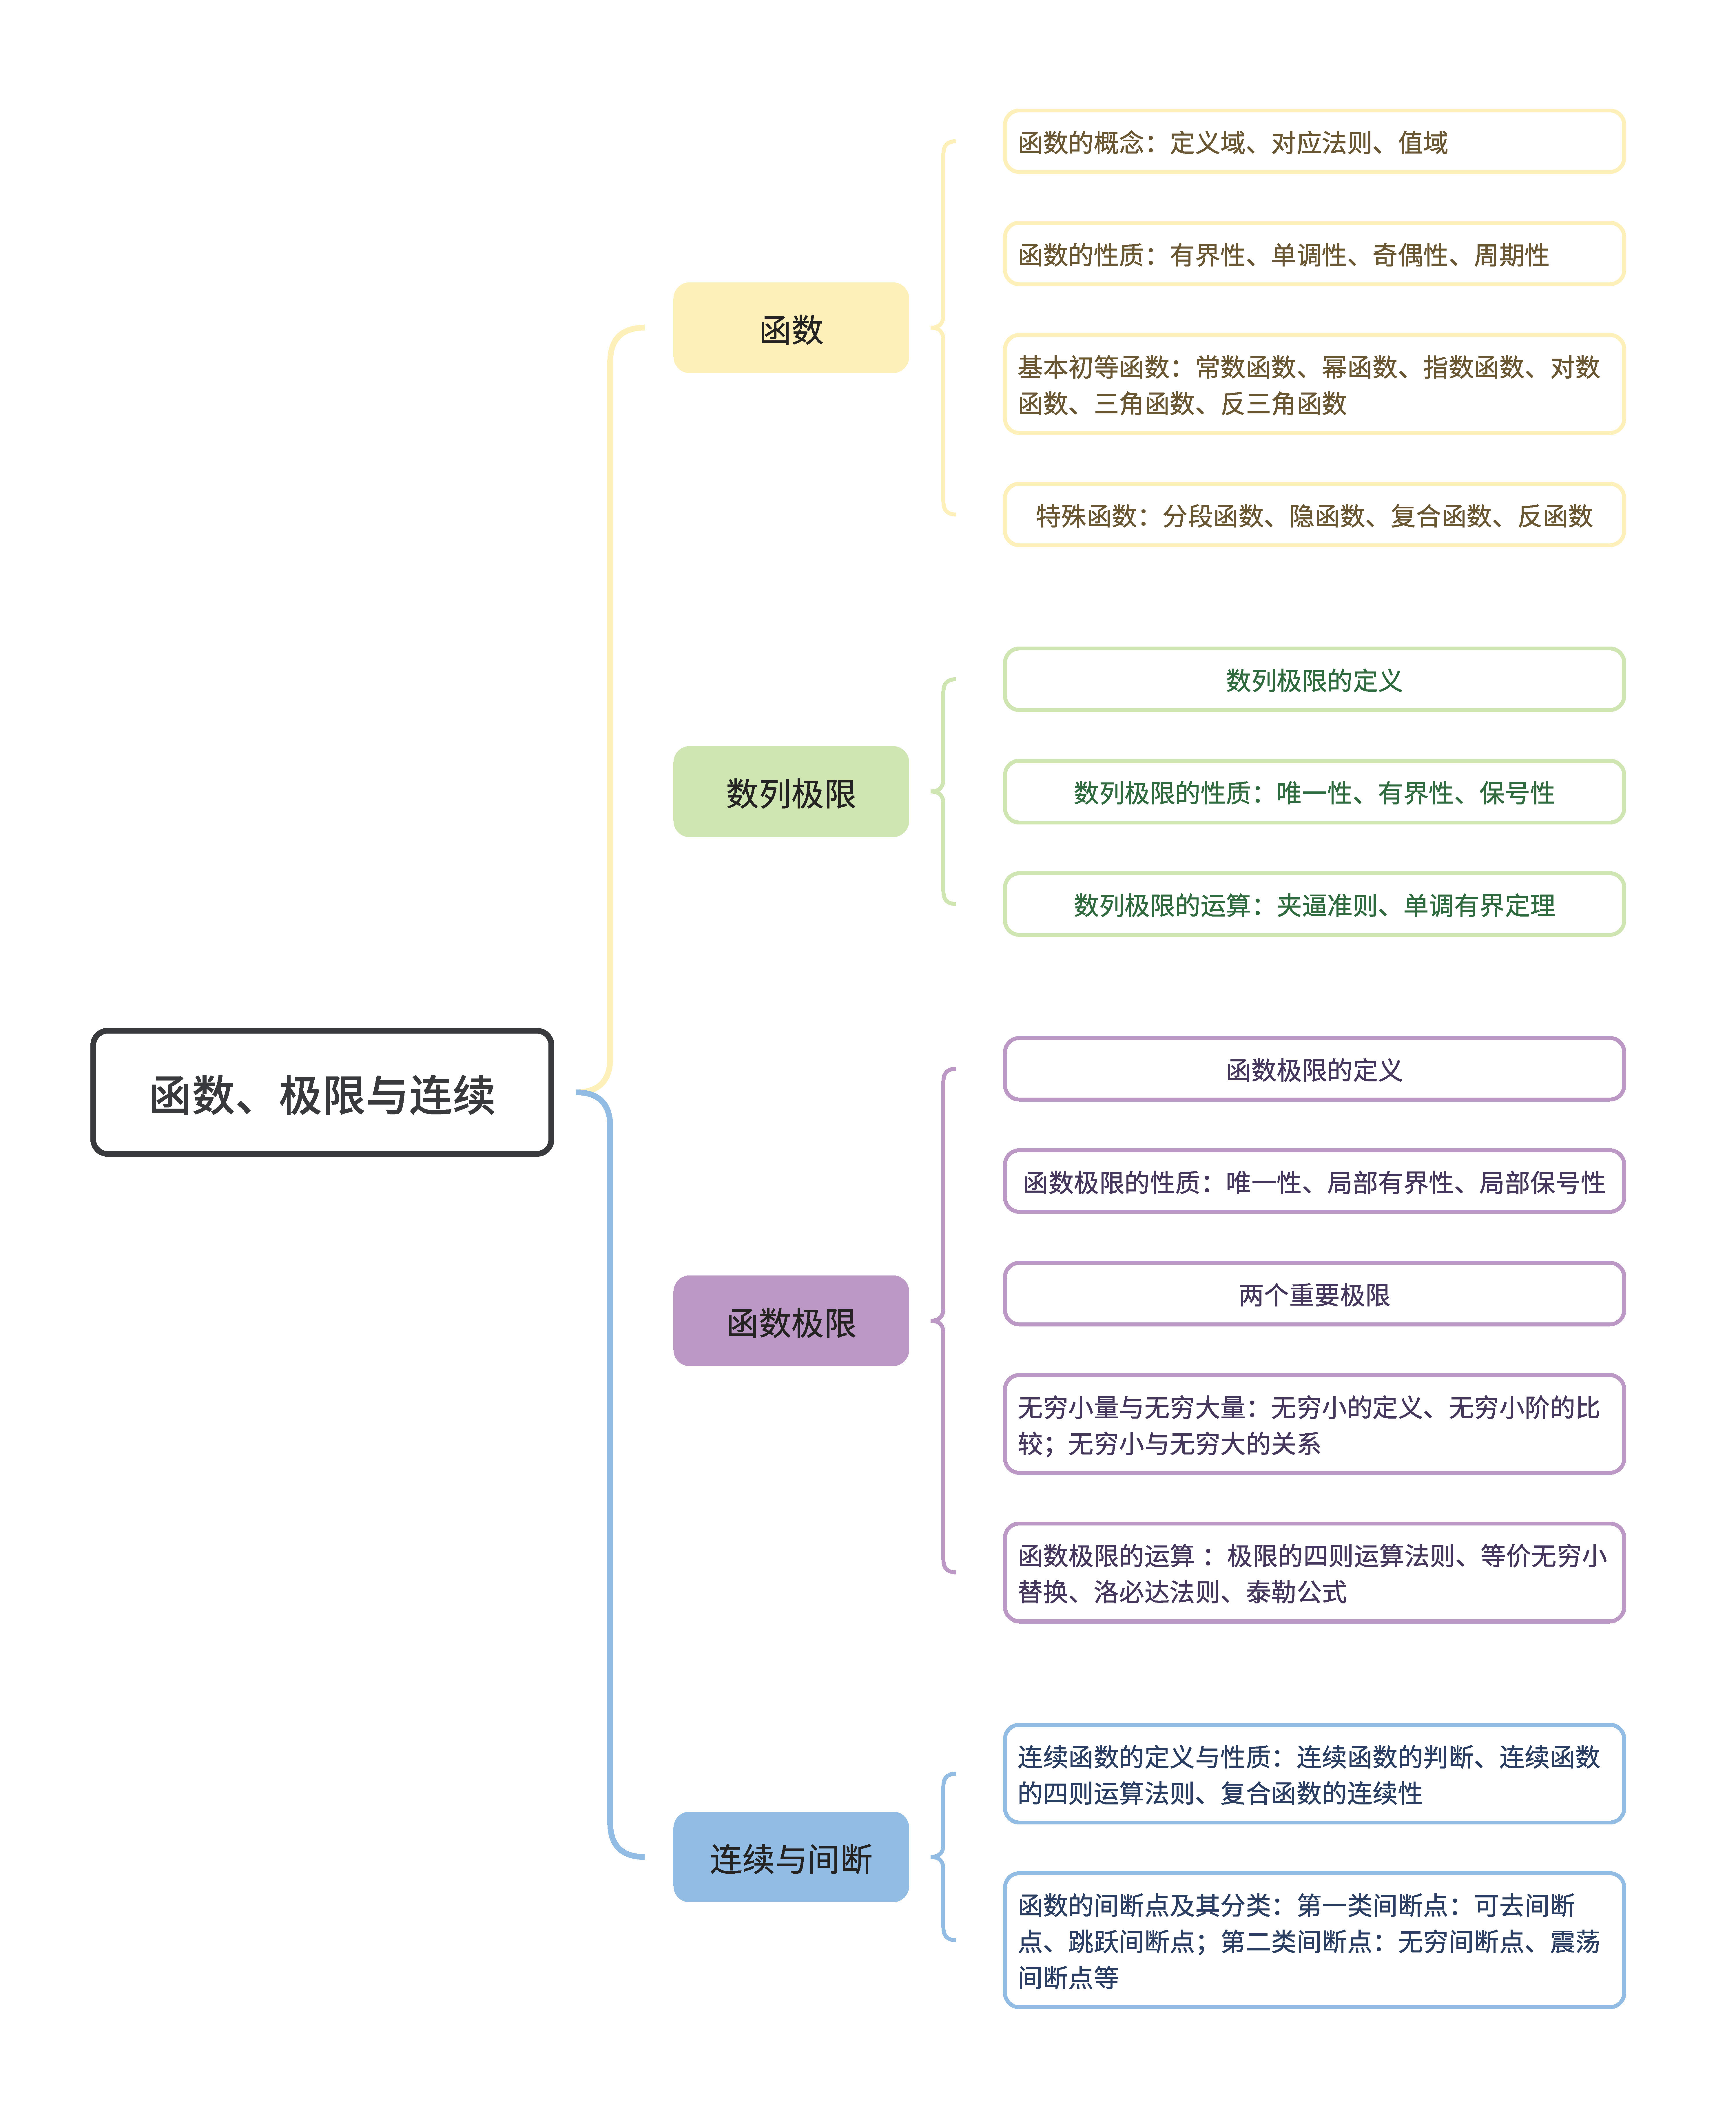
\includegraphics[width=6cm]{figure/chapter/chapter1.jpg}

\section{导数}
\subsection{导数的定义}
\subsection{导数的计算}



\section{微分}


\section{导数应用}
\subsection{函数的单调性}
\subsection{函数的极值与最值}
\subsection{函数的凹凸性与拐点}
\subsection{渐近线、曲率与曲率半径}



%第3章 一元函数积分学
\include{tex/3.tex}
%第4章 多元函数微分学
\include{tex/4.tex}

%% ------------线代部分-------------%%
%第5章 行列式
\include{tex/5.tex}
%第6章 矩阵
\include{tex/6.tex}
%第7章 向量组
\include{tex/7.tex}
%第8章 方程组
\chapter{方程组}

\begin{introduction}
	\item 预备知识
	\item 数列极限
	\item 函数极限
	\item 连续与间断
\end{introduction}

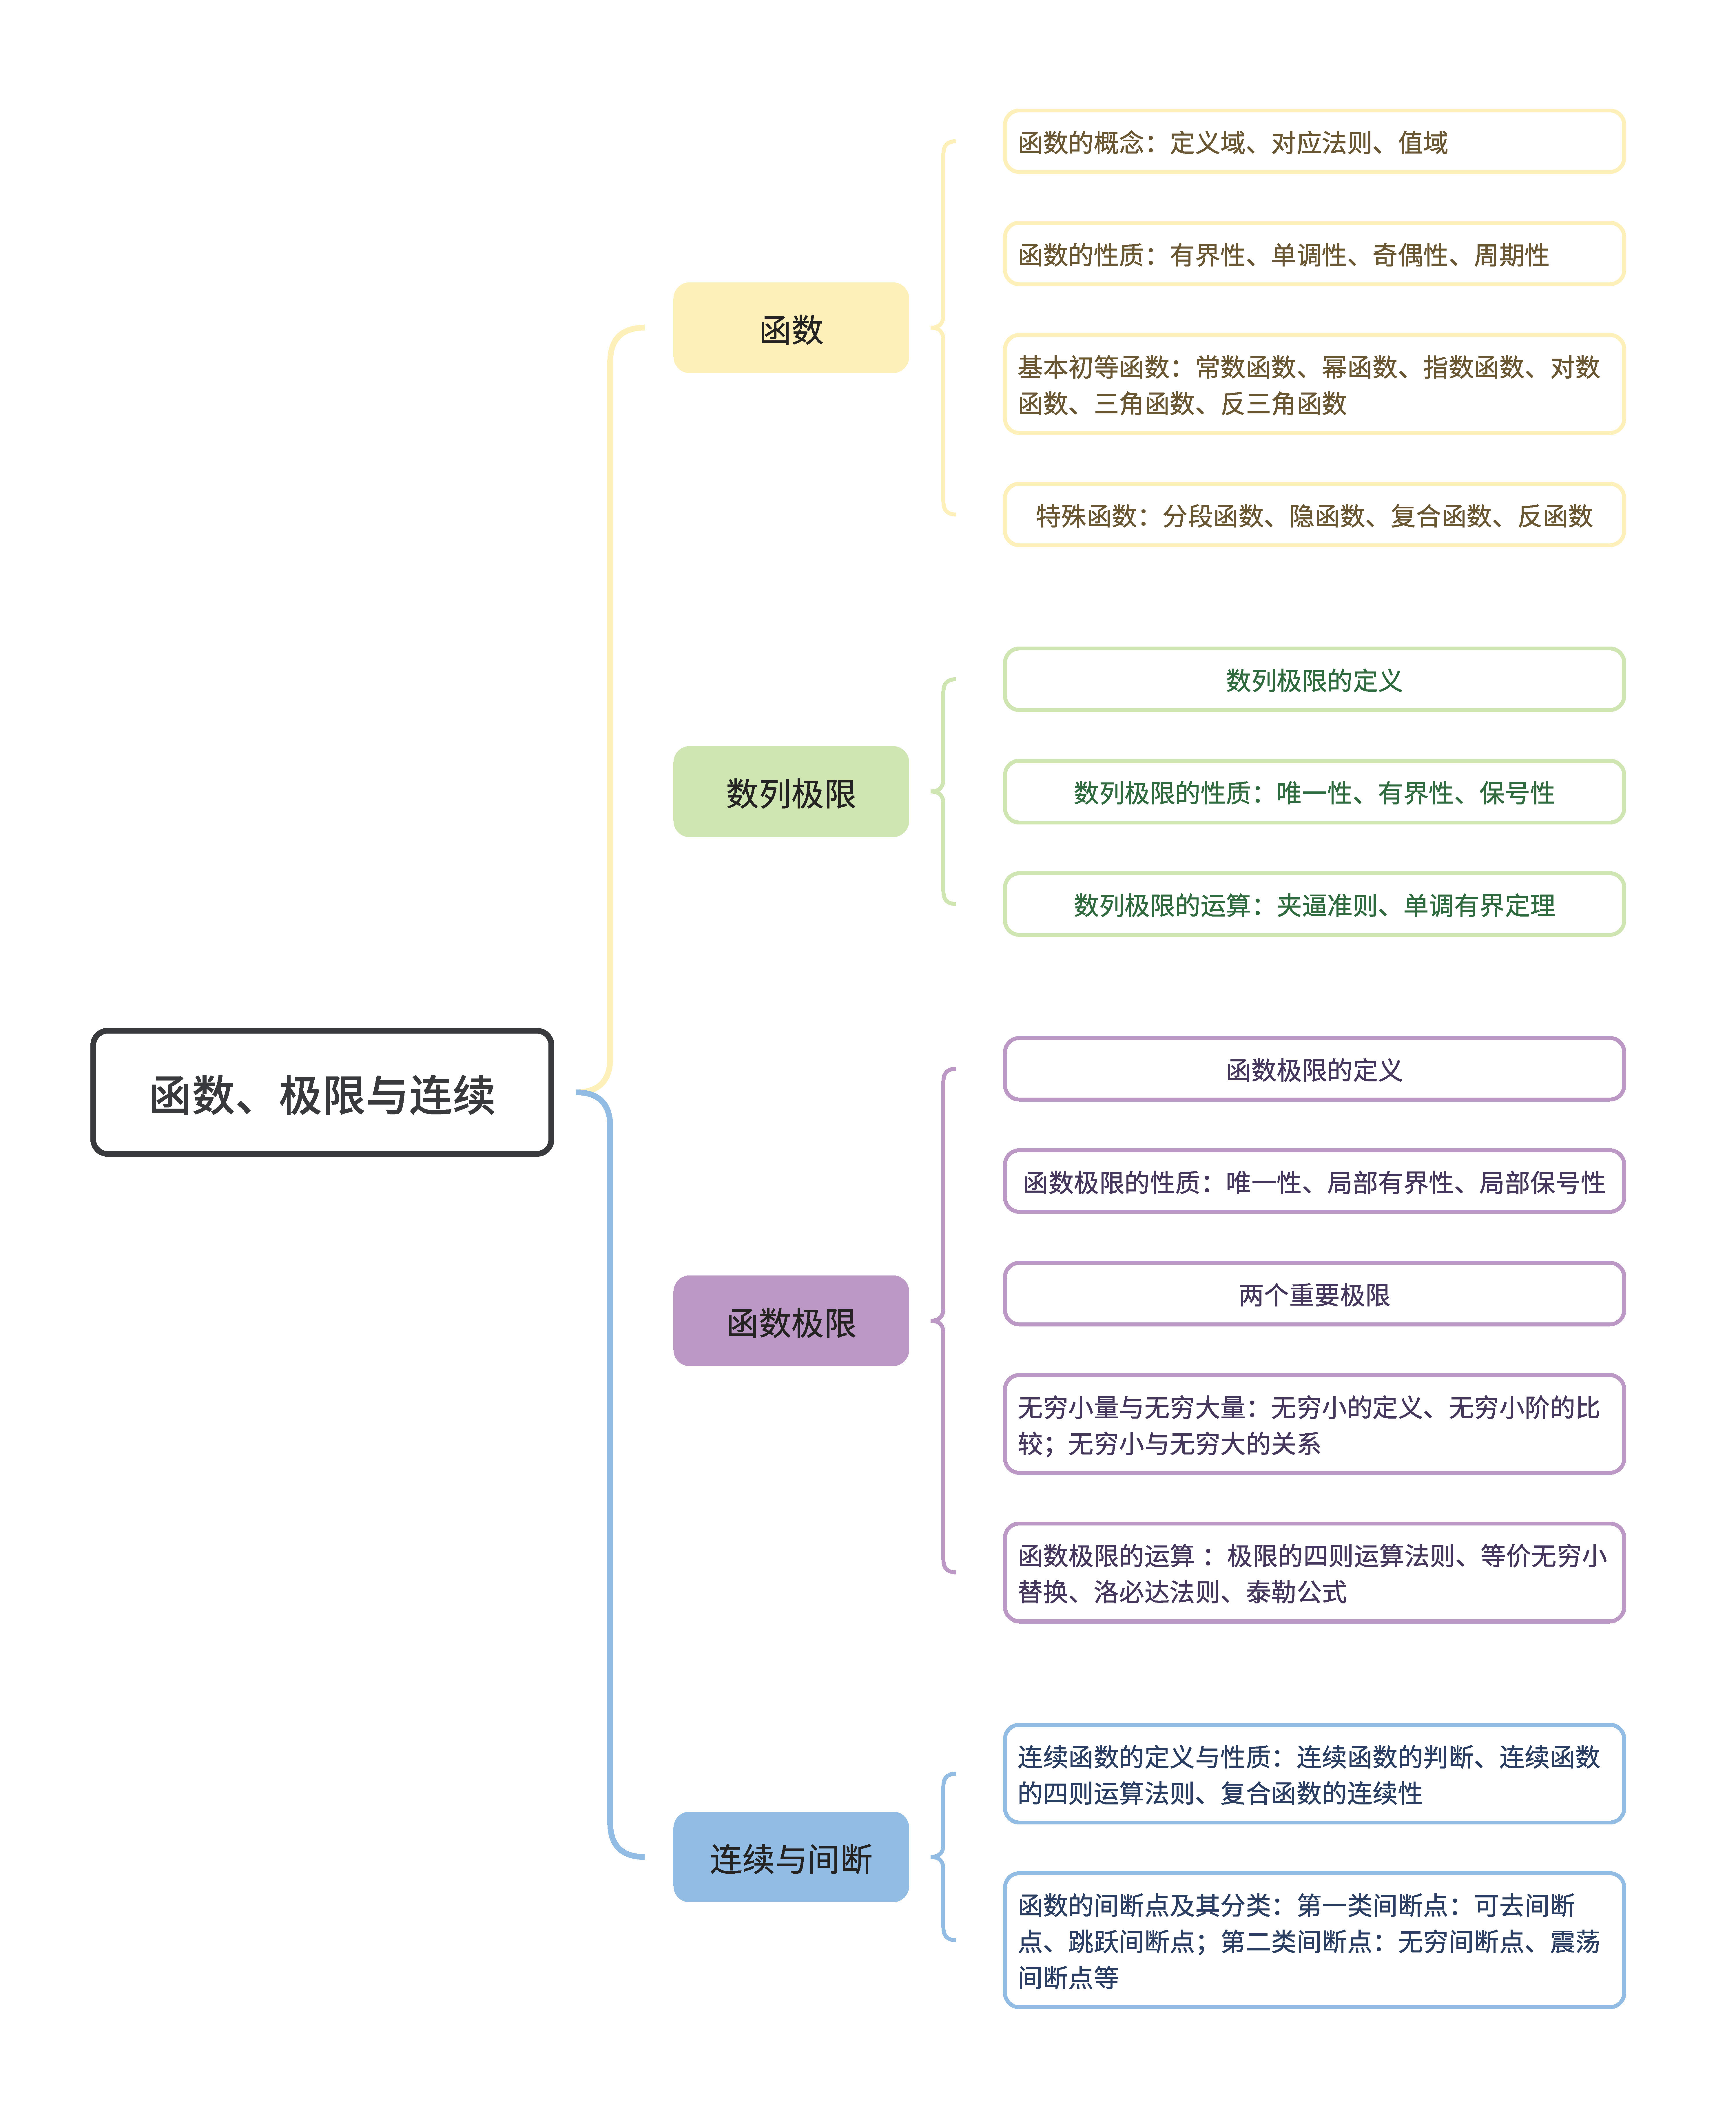
\includegraphics[width=6cm]{figure/chapter/chapter1.jpg}

\section{函数、极限与连续}
\begin{exercise}

设 $P(x)=A(x-1)+B(x-1)^2+C(x-1)^3$ 是函数 $f(x)=x^x-1$ 在点 $x=1$ 处的三阶泰勒多项式，则\fillparen[ ]
	\begin{choices}[columns=5,label-align=center]
		\item 1
		\item 2
		\item 3
		\item 4
		\item 5
	\end{choices}
	
\end{exercise}

\begin{example}	
	设 $P(x)=A(x-1)+B(x-1)^2+C(x-1)^3$ 是函数 $f(x)=x^x-1$ 在点 $x=1$ 处的三阶泰勒多项式，则\fillparen[ ]
	\begin{choices}[columns=5,label-align=center]
		\item 1
		\item 2
		\item 3
		\item 4
		\item 5
	\end{choices}
	
\end{example}






%% ------------概率部分-------------%%
%第9章 随机事件及概率
\include{tex/9.tex}
%第10章 随机变量及其分布
\include{tex/10.tex}
%第11章 随机变量的数字特征
\include{tex/11.tex}


\end{document}
